%Chapter 3

\chapter{System Architecture} % Main chapter title

\label{sysArch} % For referencing the chapter elsewhere, use \ref{Chapter7} 

\lhead{Chapter 3. \emph{System Architecture}} % This is for the header on each page - perhaps a shortened title

%----------------------------------------------------------------------------------------
\section{Overall system architecture}
In this section we provide an overall explanation of our system.  Initially, we tried to explore different techniques and approaches for applying Semantic Similarity on Arabic text. The Semantic Similarity is then used as a affinity (similarity distance) between documents which allowed clustering documents into categories. We applied different clustering algorithms to news articles. The results of clustering news articles are then used to feed a recommendation system. The recommendation system role appears in combining the user profile and the results of the clusters to recommend articles to the user that probably will be of interest to him. Figure \ref{fig:arch_1} shows the overall system architecture.
The rest of the chapter is organized as follows section ~\ref{sec:crowlers} describe the module that retrieve different documents from different sources. The preprocessing of the documents is showed in section ~\ref{sec:preprocessing}, after preprocessing one of similarity metrics is used as showed in section ~\ref{sec:similarity}

\begin{figure}[htb]
\begin{center}
%left,bottom,right,top
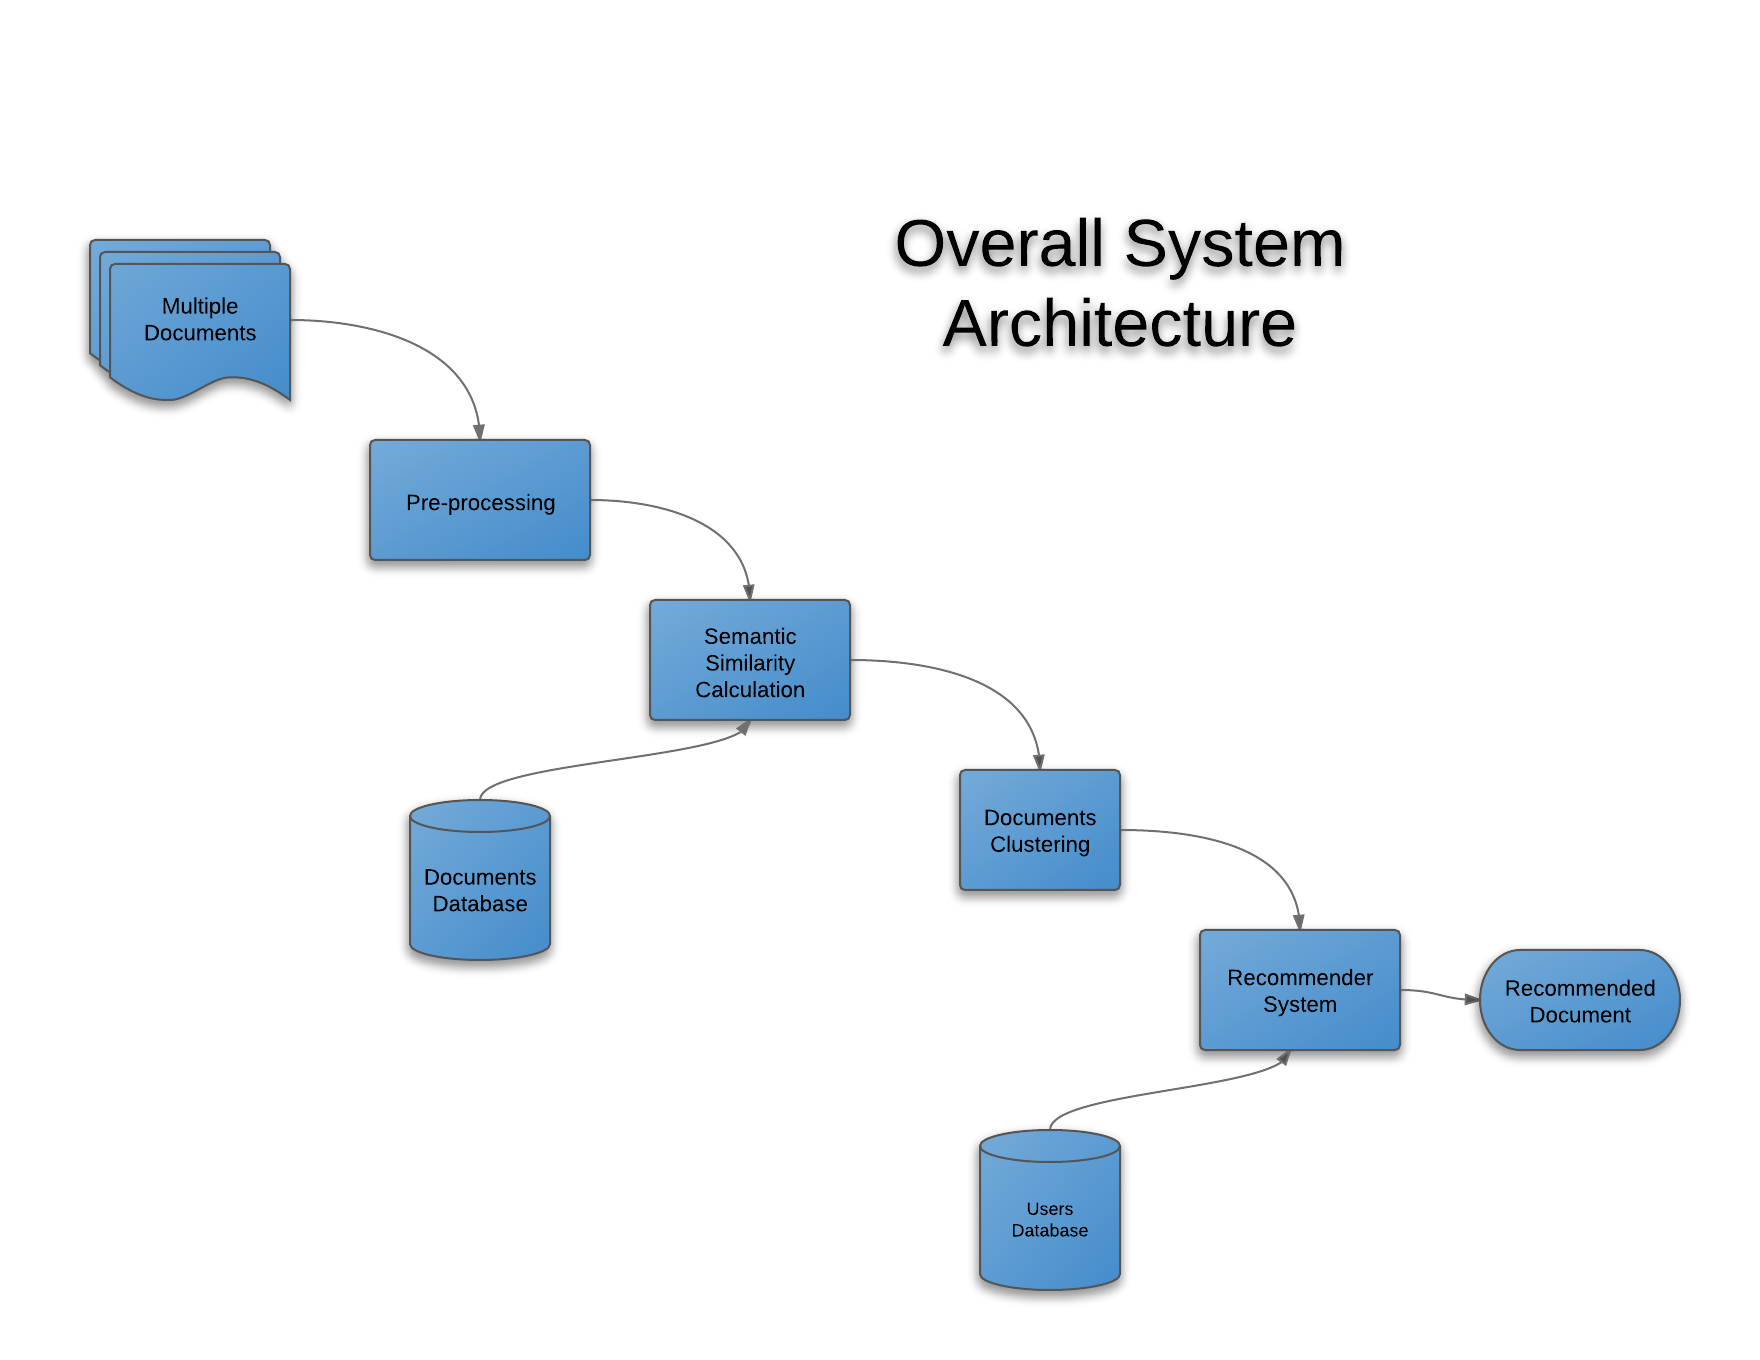
\includegraphics[totalheight=.5\textheight,
width=1\textwidth]{./Figures/arch_1.png}
\end{center}
\caption{Overall System Architecture}
\label{fig:arch_1}
\end{figure}



\section{Web crawlers}\label{sec:crowlers}
A part of our system is collecting the news articles that will be later processed. An approach would be manually feeding the system with these articles. However, this approach has a very low throughput and scalability with respect to the tremendous increase in the news streams day after day. A more practical approach is autonomous web crawlers that starts at some URL and then moves to all the outgoing links. Web crawlers also parses the web page and extracts the textual content which will be later processed. In our system we used Web Harvest [REF Web Harvest in tools section] project. Web Harvest, given a parsing XML file and some starting URLs, starts the crawling process at the starting URLs. Web Harvest parses the web page according to the given XML file and extracts all the URLs in the current page, URLs that belong to the same domain name as the page being processed, it saves the page content to an external directory and moves to the new URLs. The web pages’ content that the crawler saved is then fed into the preprocessing module of the system for further processing.
\section{Preprocessing}\label{sec:preprocessing}
After each document is retrieved some pre-processing is performed, where each term is assigned a part of speech tag(POS), then stop words are removed where a whitlist of stopwords is used(it contains the words that occur in most of documents) after this step each document will be represented by a vector of terms and the corresponding POS, this vector is used in the stemming step, where each term is first normalized by removing diacritics then one of two stemmer is used (i)Elkhoja stemmer (ii)Light stemmer).Figure ~\ref{fig:arch_1} shows the overall architecture of the system
The final representation of the document is obtained by concatinating the term to its POS as showed in figure ~\ref{fig:arch_3}.

\begin{figure}[htb]
\begin{center}
%left,bottom,right,top
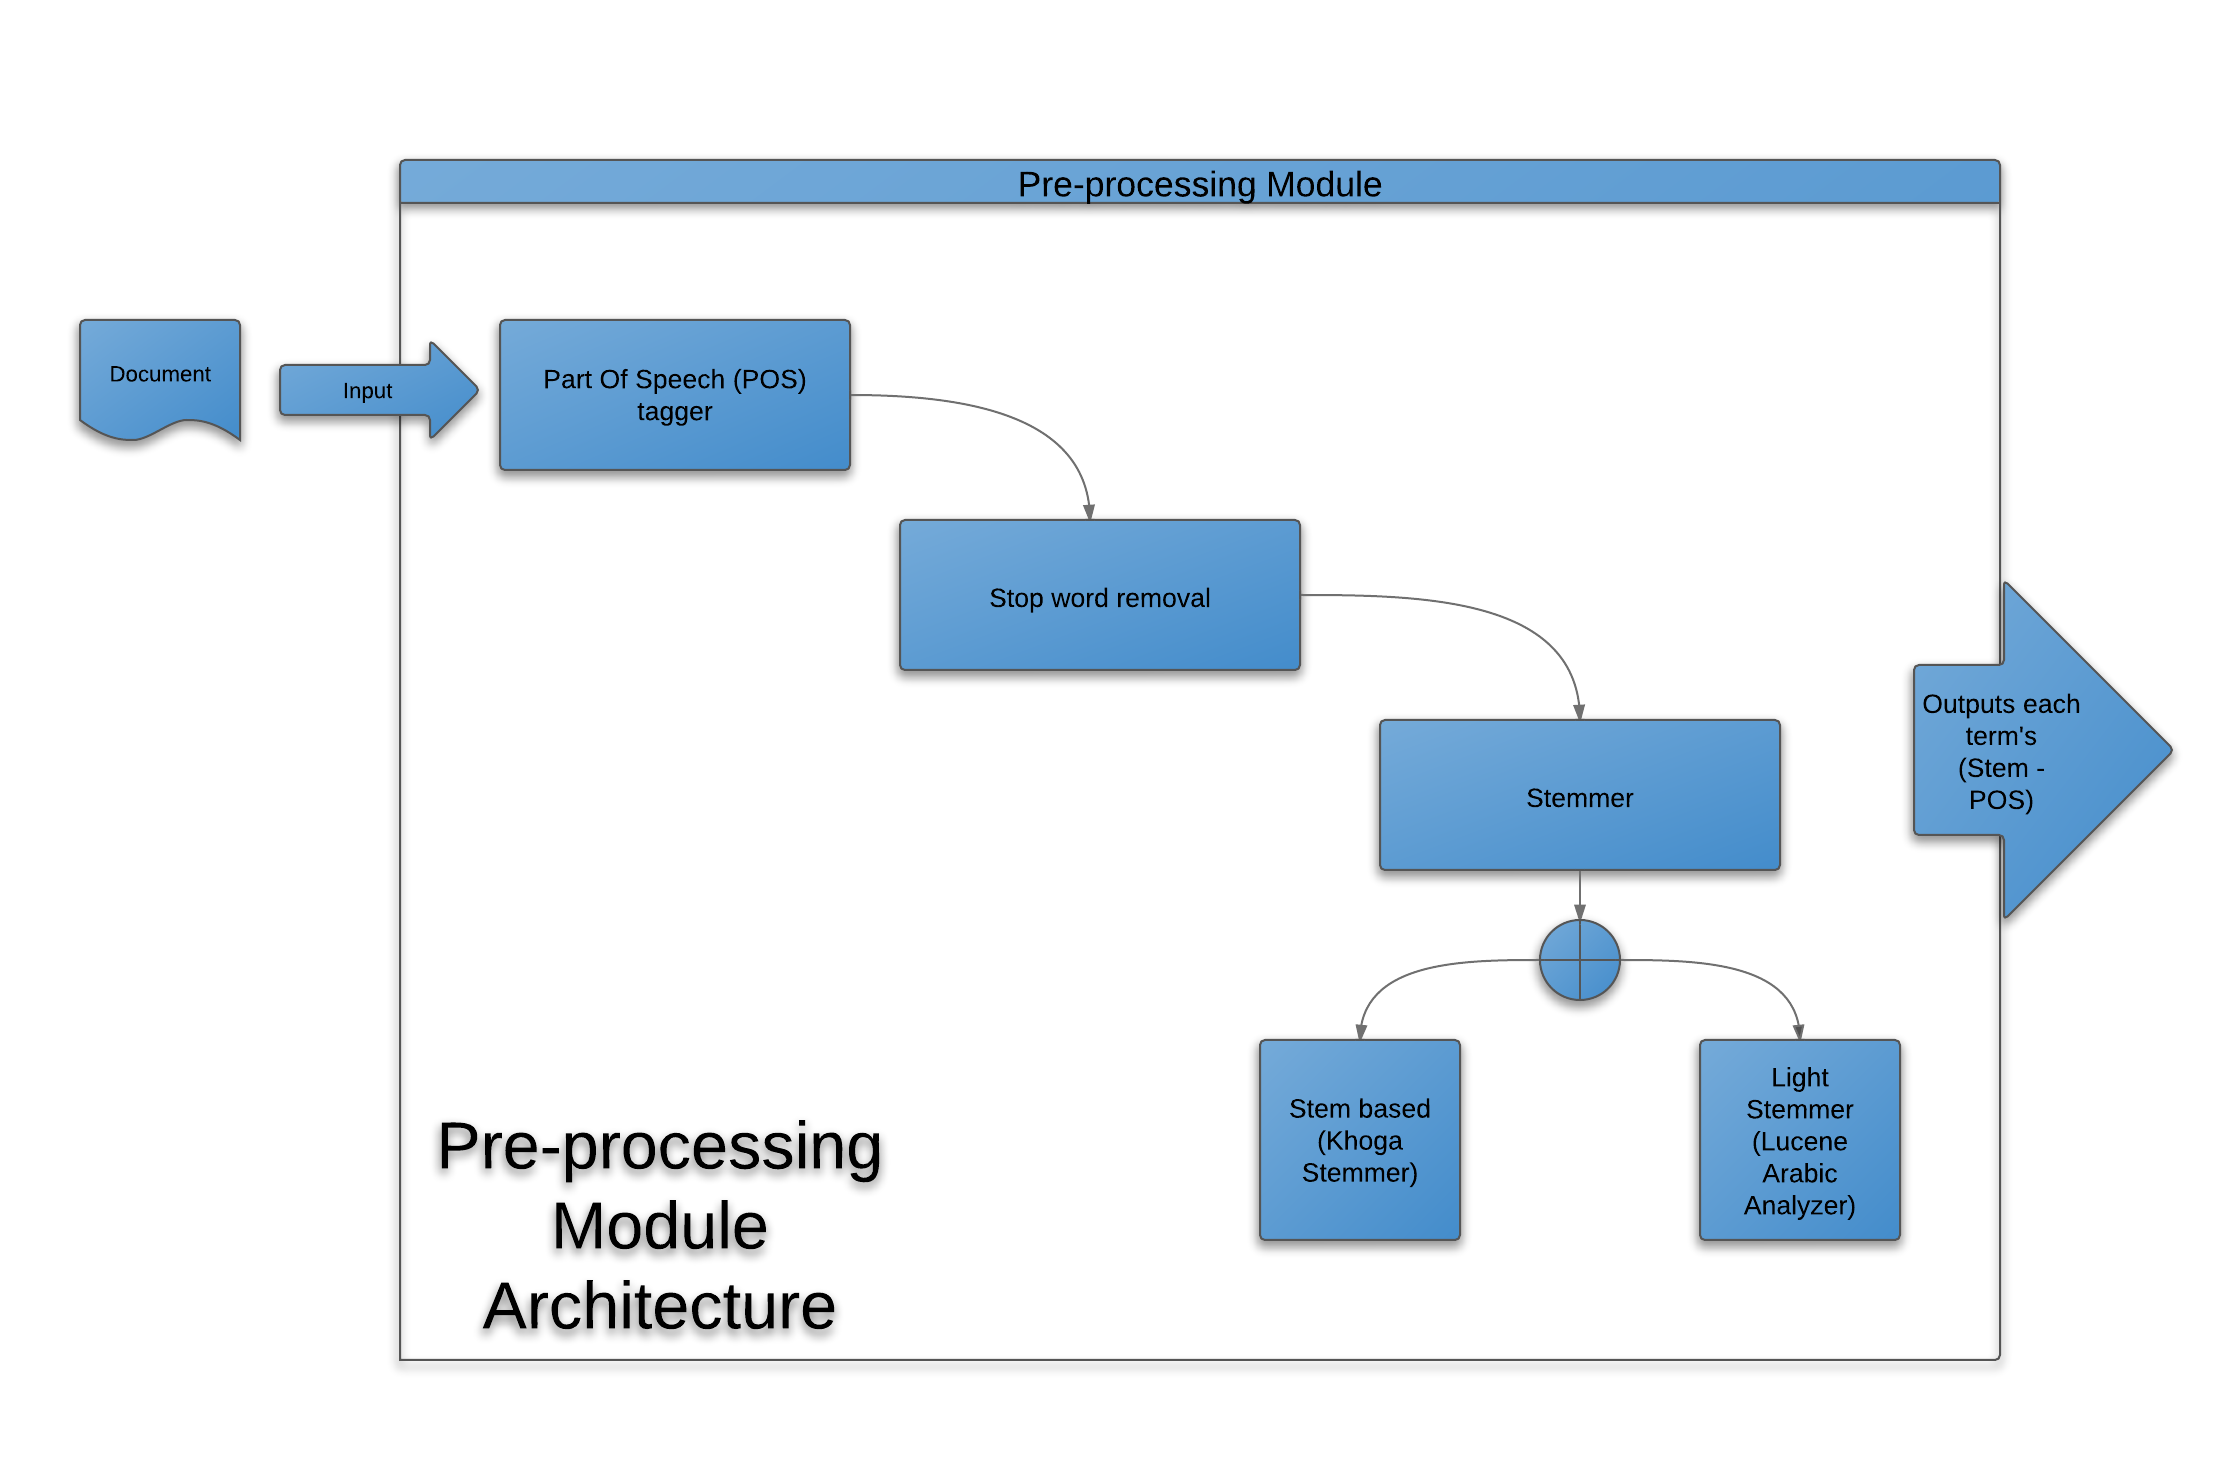
\includegraphics[totalheight=1\textheight,
width=1\textwidth]{./Figures/arch_2.png}
\end{center}
\caption{Preprocessing Module}
\label{fig:arch_2}
\end{figure}


\begin{figure}[htb]
\begin{center}
%left,bottom,right,top
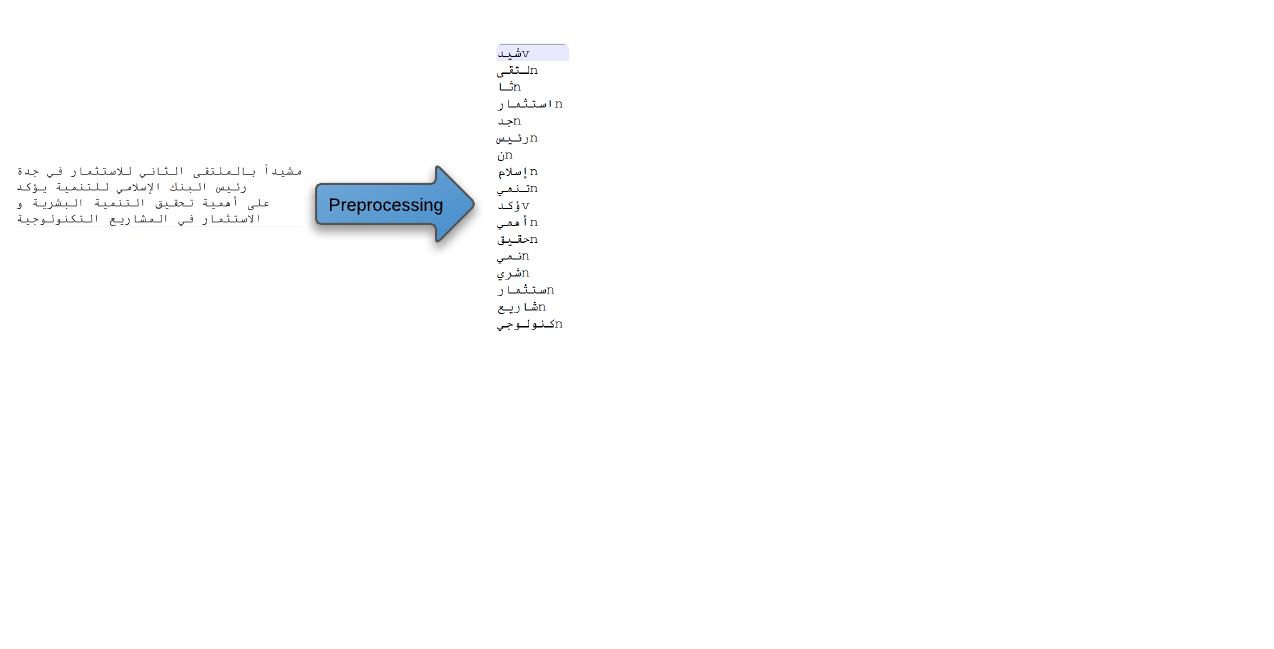
\includegraphics[totalheight=.75\textheight,
width=.75\textwidth]{./Figures/arch_3.png}
\end{center}
\caption{Example of preprocessing}
\label{fig:arch_3}
\end{figure}

\section{Similarity Module}~\label{sec:similarity}
A core module of our system is the \textit{similarity module}. In the similarity module we examined various approaches. First we examined the lexical similarity approach where each document is represented by a vector of terms in which each cell in this vector represents the TF-IDF value for this term in the document and the input corpus. 
Finally, Document-to-Document similarity is calculated using cosine similarity measure by comparing the vectors of terms representing each document.

Then we examined the Semantic Similarity approach. Here we investigated the two major approaches the Corpus based and the knowledge based.

\subsection{Corpus based}
For the corpus based we chose to work with the Latent Semantic Analysis (LSA) to calculate the semantic similarity between two given documents. The documents collected are then represented using the term-by-document matrix. In the term-by-document matrix every column vector represents a document and every row represents a term that occurred at least once in the whole corpus. Every cell in the document vector represents the frequency by which the corresponding term appeared in that document. In other words, the term-by-document matrix represents the TF-IDF of the term of the whole corpus and the documents in the corpus. Another way to think of this is that LSA represents the meaning of a word as a kind of average of the meaning of all the documents in which it appears, and the meaning of a document as a kind of average of the meaning of all the words it contains.
Next we apply Singular Value Decomposition (SVD), a well known operation in Linear Algebra. This step is used to lower the dimensionality of the term-by-document matrix.
After that we represent each document as the mean of the vectors of the terms that appeared in this document. And for any two given documents we can calculate the semantic similarity by calculating the Cosine Similarity between their vectors.

\subsection{Knowledge based}
Here we used Arabic WordNet as Ontology to calculate the Document-to-Document Similarity we used the Wu-Palmer techniques as it utilizes the existence of the hierarchical of the Ontology to great extent.
AWN lacks to any performance optimization for example it took around 15 min. to computer single Document-to-Document Similarity, this performance forced us to modify the AWN core a little bit so we managed to decrease the running time to reach the range of 3-4 min.. Unfortunately this wasn’t good enough as our system target domain is characterized by the high dynamicity of the dataset which makes it difficult to cope with it using AWN poor performance.
Next, we thought about using Wikipedia as an Ontology due to its tremendous growth, so we investigate the Semantic Similarity approaches related to Wikipedia.There are many approaches but we used only 2 of them, First one uses wikipedia Articles each as a new Concept, using some inverted index on all the article, we could find the specific Concept(articles) where any term appeared, collecting these results in a global vector and finally perform cosine similarity measure.
Second one used the categories of the wikipedia articles instead of the wikipedia article itself, and the rest like the previous one.

\section{Document clustering}
Using the simialrity metric explained in the previous section different clustering algorithms can be applied to group the similar document or neighbour users to increase the system scalability.

The pairwise similarity between documents is stored in a database and is fed to the clustering algorithm, one of the clustering algorithms showed in chapter ~\ref{clustering} is used to assign a cluster ID to each document.
Mitosis clustering algorithm which explained in chapter ~\ref{clustering} is used to cluster document and users

\section{Recommender system}
\subsection{Recommending Approach}
We have implemented the recommender using collaborative via content approach (chapter ~\ref{recommender}) where users profile are build using the content based representation of their rated items.

As illustrated in figure ~\ref{fig:reco_1}, the user profile is examined against the user's neighbour and the correlation between the user and each of his neighbours is calculated and stored in a database for a certain time then it expires and has to be updated as the taste of the user may deviate than the current neighbours. where users profile are build using the content based representation of their rated items, the profile is saved in an array of fixed width (LSA concepts number). The document metadata is saved in the documents table while its vector representation is derived from the LSA's term vs. document matrix.
The system obtains the items read by user's neighbours and not read by the user (potential interesting items). 
Based on the correlation and neighbour's rate for the new documents the system can rank the documents and show the top $N$ recommendations to the user.
After showing the recommendations to the user the system measures the user \textit{feedback} implicitly by watching the time the user read a document and compare it to its average reading time, if it is bigger than the average so it will be considered as positive feedback. Sharing a document implies being interested in it and therefore will be considered as a positive feedback, also there exist a like and dislike option which implies positive and negative feedback respectively. this feedback to update the user's profile based on this feedback and document content.
\begin{figure}[htb]
\begin{center}
%left,bottom,right,top
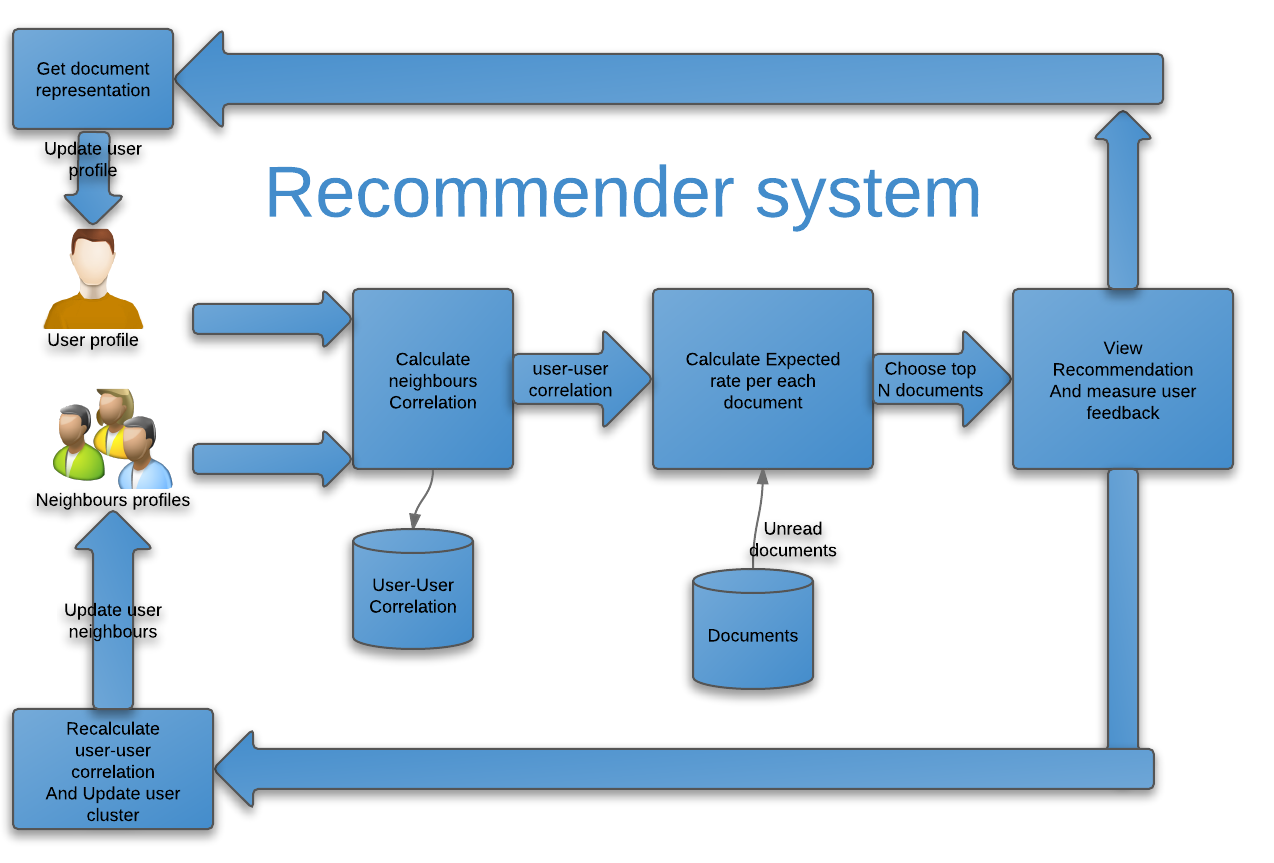
\includegraphics[totalheight=1\textheight,
width=1\textwidth]{./Figures/reco_1.png}
\end{center}
\caption{Overview of Recommender system}
\label{fig:reco_1}
\end{figure}

\subsection{User's correlation}
Correlation between users is time stamped so that we don't have to recalculate the correlation every time a recommendation is required and in case invalidation occurs i.e. the time stamp period has expired, correlation is recalculated again and then clustering is applied to keep track of the user's taste change.
User's recommendations are saved in database in order to avoid recommending a seen item again to the user. Figure ~\ref{fig:reco_2} shows the ERD of the database used.

\subsection{User Profile}
Each user is represented by a vector similar to that of the document where both of them have the same length that is equal to the number of documents in the corpus used in performing LSA
\subsection{User's neighbors}
When a user enters the system a user profile is created then these profile is fed with his social activates. The user profile is compared to other users profile using person's correlation or cosine similarity, and then users are clustered based on these similarities.
\subsection{Get Recommendations}
After determining user's cluster, documents that have been rated by the neighbors and not by that user. The expected rating of the user to the unseen documents is then calculated using a combination between user's votes and their correlation to that particular user, then top N documents with highest expected rating are chosen to be recommended to the user.


\begin{figure}[htb]
\begin{center}
%left,bottom,right,top
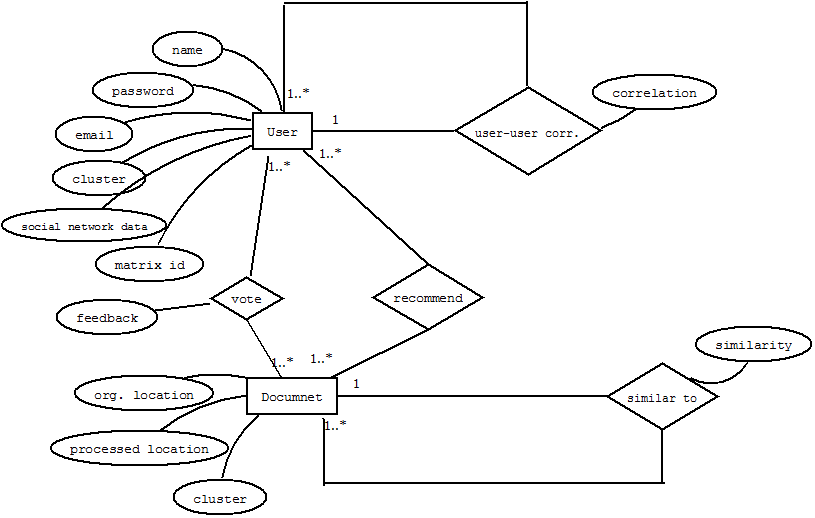
\includegraphics[totalheight=.75\textheight,
width=.75\textwidth]{./Figures/reco_2.png}
\end{center}
\caption{ERD of Recommender system}
\label{fig:reco_2}
\end{figure}

{Document Representation}
Each document in the system is represented as a vector of concepts. These vectors are driven by aggregating the vector representing words placed in the document via LSA's term vs. document matrix 
\section{User Profile}
Each user is represented by a vector similar to that of the document where both of them have the same length that is equal to the number of documents in the corpus used in performing LSA
\section{User's neighbors}
When a user enters the system a user profile is created then these profile is fed with his social activates. The user profile is compared to other users profile using person's correlation or cosine similarity, and then users are clustered based on these similarities.
\section{Get Recommendations}
After determining user's cluster, documents that have been rated by the neighbors and not by that user. The expected rating of the user to the unseen documents is then calculated using a combination between user's votes and their correlation to that particular user, then top N documents with highest expected rating are chosen to be recommended to the user.

